\documentclass{article}\usepackage[]{graphicx}\usepackage[]{color}
%% maxwidth is the original width if it is less than linewidth
%% otherwise use linewidth (to make sure the graphics do not exceed the margin)
\makeatletter
\def\maxwidth{ %
  \ifdim\Gin@nat@width>\linewidth
    \linewidth
  \else
    \Gin@nat@width
  \fi
}
\makeatother

\definecolor{fgcolor}{rgb}{0.345, 0.345, 0.345}
\newcommand{\hlnum}[1]{\textcolor[rgb]{0.686,0.059,0.569}{#1}}%
\newcommand{\hlstr}[1]{\textcolor[rgb]{0.192,0.494,0.8}{#1}}%
\newcommand{\hlcom}[1]{\textcolor[rgb]{0.678,0.584,0.686}{\textit{#1}}}%
\newcommand{\hlopt}[1]{\textcolor[rgb]{0,0,0}{#1}}%
\newcommand{\hlstd}[1]{\textcolor[rgb]{0.345,0.345,0.345}{#1}}%
\newcommand{\hlkwa}[1]{\textcolor[rgb]{0.161,0.373,0.58}{\textbf{#1}}}%
\newcommand{\hlkwb}[1]{\textcolor[rgb]{0.69,0.353,0.396}{#1}}%
\newcommand{\hlkwc}[1]{\textcolor[rgb]{0.333,0.667,0.333}{#1}}%
\newcommand{\hlkwd}[1]{\textcolor[rgb]{0.737,0.353,0.396}{\textbf{#1}}}%
\let\hlipl\hlkwb

\usepackage{framed}
\makeatletter
\newenvironment{kframe}{%
 \def\at@end@of@kframe{}%
 \ifinner\ifhmode%
  \def\at@end@of@kframe{\end{minipage}}%
  \begin{minipage}{\columnwidth}%
 \fi\fi%
 \def\FrameCommand##1{\hskip\@totalleftmargin \hskip-\fboxsep
 \colorbox{shadecolor}{##1}\hskip-\fboxsep
     % There is no \\@totalrightmargin, so:
     \hskip-\linewidth \hskip-\@totalleftmargin \hskip\columnwidth}%
 \MakeFramed {\advance\hsize-\width
   \@totalleftmargin\z@ \linewidth\hsize
   \@setminipage}}%
 {\par\unskip\endMakeFramed%
 \at@end@of@kframe}
\makeatother

\definecolor{shadecolor}{rgb}{.97, .97, .97}
\definecolor{messagecolor}{rgb}{0, 0, 0}
\definecolor{warningcolor}{rgb}{1, 0, 1}
\definecolor{errorcolor}{rgb}{1, 0, 0}
\newenvironment{knitrout}{}{} % an empty environment to be redefined in TeX

\usepackage{alltt}
\usepackage[sc]{mathpazo}
\usepackage[T1]{fontenc}
\usepackage{geometry}
\geometry{verbose,tmargin=2.5cm,bmargin=2.5cm,lmargin=2.5cm,rmargin=2.5cm}
\setcounter{secnumdepth}{2}
\setcounter{tocdepth}{2}
\usepackage{url}
\usepackage[unicode=true,pdfusetitle,
 bookmarks=true,bookmarksnumbered=true,bookmarksopen=true,bookmarksopenlevel=2,
 breaklinks=false,pdfborder={0 0 1},backref=false,colorlinks=false]
 {hyperref}
\hypersetup{
 pdfstartview={XYZ null null 1}}
\usepackage{breakurl}
\IfFileExists{upquote.sty}{\usepackage{upquote}}{}
\begin{document}


\title{Car Evaluation Dataset - CM3111}
\author{Muhammed Umair Iqbal}
\maketitle
\section{Data Exploration}
\subsection{Dataset Choice}
I have selected a data set that is related to cars as I have a passion for cars and thought that it would be a good exploring a data set related to cars via R Studio. I got my dataset from the UCI Machine Learning Repository from "http://archive.ics.uci.edu/ml/datasets/Car+Evaluation".
\subsection{Technology Platform}
The application I have used to explore my data is R Studio and carry out experiments on. After researching hadoop i have found that i do not need to be using it. For many reasons, one of them being that Hadoop can store massive amounts of data, Petabytes to be exact. Moreover Hadoop should be used when the users requires thousands of operations per second on terabytes of data at a time, which is not what is required in this instance which is why i haven't incorporated Hadoop or any other Big Data Technologies.

\subsection{Problem Statement}

The dataset I have choosen is a Car Evaluation dataset.It has 6 Attributes;
\begin{itemize}
\item Price
\item Maint(Maintence of the car)
\item Doors(Number of Doors)
\item Persons(Number of people the car can seat at once)
\item Boot(The size of the boot)
\item Safety(The safety rating of the car)
\end{itemize}
The aim is to build a predictive model, to predict what the Evaluation is of the car.
\subsection{Data Exploration} 
I began to explore my Data set, by finding out the numbers of rows and coloumns
\begin{knitrout}
\definecolor{shadecolor}{rgb}{0.969, 0.969, 0.969}\color{fgcolor}\begin{kframe}
\begin{alltt}
\hlcom{#Seting working directory}
    \hlstd{curdir} \hlkwb{<-} \hlkwd{getwd}\hlstd{()}
\hlcom{#Reading in my prefered dataset(Calling it df for short of Data frame)}
  \hlstd{df}\hlkwb{=}\hlkwd{read.csv}\hlstd{(}\hlkwd{paste}\hlstd{(curdir,}\hlstr{"/car.data"}\hlstd{,}\hlkwc{sep} \hlstd{=} \hlstr{""}\hlstd{),}\hlkwc{header}\hlstd{=T,}
              \hlkwc{na.strings}\hlstd{=}\hlstr{"?"}\hlstd{)}
  \hlstd{nr} \hlkwb{<-} \hlkwd{nrow}\hlstd{(df)} \hlcom{# number of rows}
  \hlstd{nc} \hlkwb{<-} \hlkwd{ncol}\hlstd{(df)} \hlcom{# number of columns}
\hlcom{#delivering the data the way i want to present it }
  \hlkwd{cat} \hlstd{(}\hlstr{"Cars Evaluation Dataset has: "}\hlstd{, nr,}\hlstr{" Rows"}\hlstd{,} \hlstr{" and "}\hlstd{,nc,} \hlstr{" Columns"}\hlstd{)}
\end{alltt}
\begin{verbatim}
## Cars Evaluation Dataset has:  1727  Rows  and  7  Columns
\end{verbatim}
\end{kframe}
\end{knitrout}
I then got a breif description from R before changing making any changes to the dataset
\begin{knitrout}
\definecolor{shadecolor}{rgb}{0.969, 0.969, 0.969}\color{fgcolor}\begin{kframe}
\begin{alltt}
\hlcom{#Reciveing a breif description of the data set}
  \hlkwd{str}\hlstd{(df)}
\end{alltt}
\begin{verbatim}
## 'data.frame':	1727 obs. of  7 variables:
##  $ vhigh  : Factor w/ 4 levels "high","low","med",..: 4 4 4 4 4 4 4 4 4 4 ...
##  $ vhigh.1: Factor w/ 4 levels "high","low","med",..: 4 4 4 4 4 4 4 4 4 4 ...
##  $ X2     : Factor w/ 4 levels "2","3","4","5more": 1 1 1 1 1 1 1 1 1 1 ...
##  $ X2.1   : Factor w/ 3 levels "2","4","more": 1 1 1 1 1 1 1 1 2 2 ...
##  $ small  : Factor w/ 3 levels "big","med","small": 3 3 2 2 2 1 1 1 3 3 ...
##  $ low    : Factor w/ 3 levels "high","low","med": 3 1 2 3 1 2 3 1 2 3 ...
##  $ unacc  : Factor w/ 4 levels "acc","good","unacc",..: 3 3 3 3 3 3 3 3 3 3 ...
\end{verbatim}
\end{kframe}
\end{knitrout}
The coloumns of the dataset can be dislayed by doing the following:
\begin{knitrout}
\definecolor{shadecolor}{rgb}{0.969, 0.969, 0.969}\color{fgcolor}\begin{kframe}
\begin{alltt}
\hlcom{#Retrieving the coloumn names}
  \hlkwd{names}\hlstd{(df)}
\end{alltt}
\begin{verbatim}
## [1] "vhigh"   "vhigh.1" "X2"      "X2.1"    "small"   "low"     "unacc"
\end{verbatim}
\end{kframe}
\end{knitrout}
\subsubsection{The Class distribution in the dataset is the Evaluation }
\begin{table}[ht]
\caption{Number of Instances per Class} % title of Table
\centering % used for centering table
\begin{tabular}{c c c } % centered columns (3 columns)
\hline\hline %inserts double horizontal lines
Class & Number & Number as a Percentage \\ [0.5ex] % inserts table
%heading
\hline % inserts single horizontal line
unacc & 1210 & 70.023 \\ % inserting body of the table
acc & 348 & 22.222 \\
good & 69 & 3.993 \\
v-good & 65 & 3.769 \\ [1ex] % [1ex] adds vertical space
\hline %inserts single line
\end{tabular}
\label{table:nonlin} % is used to refer this table in the text
\end{table}
\subsubsection*{Below is the Maintence ratings in the dataset for the cars.}
\subsubsection*{Below there is also a graph with the car Price Ratings.}
\subsubsection*{Also below is a bar graph the car evaluation with their level of Acceptiblity}
\begin{knitrout}
\definecolor{shadecolor}{rgb}{0.969, 0.969, 0.969}\color{fgcolor}\begin{kframe}
\begin{alltt}
\hlcom{#Bar plot of the Maintence rating of the cars}
  \hlstd{labelFreqs} \hlkwb{<-} \hlkwd{table}\hlstd{(df}\hlopt{$}\hlstd{Maint)}\hlcom{# frequency of labels}
    \hlkwd{barplot}\hlstd{(labelFreqs,}\hlkwc{col} \hlstd{=} \hlkwd{gray.colors}\hlstd{(}\hlnum{4}\hlstd{),}\hlkwc{xlab}\hlstd{=}\hlstr{"Car Ratings"}\hlstd{,}
        \hlkwc{main}\hlstd{=}\hlstr{"Maintence Ratings"}\hlstd{)}
\hlcom{#Bar Plot of the price rating of the cars}
  \hlstd{labelFreqs} \hlkwb{<-} \hlkwd{table}\hlstd{(df}\hlopt{$}\hlstd{Price)}\hlcom{# frequency of labels}
   \hlkwd{barplot}\hlstd{(labelFreqs,}\hlkwc{col} \hlstd{=} \hlkwd{gray.colors}\hlstd{(}\hlnum{4}\hlstd{),}\hlkwc{xlab}\hlstd{=}\hlstr{"Car Ratings"}\hlstd{,}
             \hlkwc{main}\hlstd{=}\hlstr{"Price Ratings"}\hlstd{)}
  \hlstd{labelFreqs} \hlkwb{<-} \hlkwd{table}\hlstd{(df}\hlopt{$}\hlstd{Evaluation)}\hlcom{# frequency of labels}
    \hlkwd{barplot}\hlstd{(labelFreqs,}\hlkwc{col} \hlstd{=} \hlkwd{gray.colors}\hlstd{(}\hlnum{4}\hlstd{),}\hlkwc{xlab}\hlstd{=}\hlstr{"Acceptability"}\hlstd{,}
        \hlkwc{main}\hlstd{=}\hlstr{"Maintence Ratings"}\hlstd{)}
\end{alltt}
\end{kframe}
\end{knitrout}
\subsection{Pre-Processing}
Before doing anything I began by checking my data for any missing values. Moreover I was also cheking for the amount of unique values there are for each variable. I have applied a function called sapply()which is an efficient way to pass the function as an argument and apply it to
each column
\begin{knitrout}
\definecolor{shadecolor}{rgb}{0.969, 0.969, 0.969}\color{fgcolor}\begin{kframe}
\begin{alltt}
  \hlstd{na_counts} \hlkwb{<-} \hlkwd{sapply}\hlstd{(df,}\hlkwa{function}\hlstd{(}\hlkwc{x}\hlstd{)} \hlkwd{sum}\hlstd{(}\hlkwd{is.na}\hlstd{(x)))}
  \hlstd{unique_vals}\hlkwb{<-} \hlkwd{sapply}\hlstd{(df,} \hlkwa{function}\hlstd{(}\hlkwc{x}\hlstd{)} \hlkwd{length}\hlstd{(}\hlkwd{unique}\hlstd{(x)))}
  \hlstd{na_counts}
\end{alltt}
\begin{verbatim}
##   vhigh vhigh.1      X2    X2.1   small     low   unacc 
##       0       0       0       0       0       0       0
\end{verbatim}
\begin{alltt}
  \hlstd{unique_vals}
\end{alltt}
\begin{verbatim}
##   vhigh vhigh.1      X2    X2.1   small     low   unacc 
##       4       4       4       3       3       3       4
\end{verbatim}
\end{kframe}
\end{knitrout}
Now I going to begin applying changes that i feel need to be applied in order for accuring a prediction from the dataset. 
I am going to begin with creating another dataframe so i have a back up.
\begin{knitrout}
\definecolor{shadecolor}{rgb}{0.969, 0.969, 0.969}\color{fgcolor}\begin{kframe}
\begin{alltt}
\hlcom{#Creating a back up data frame called nd(New Data)}
 \hlstd{nd} \hlkwb{<-} \hlstd{df}

\hlcom{#Re-definng the coloumn names to something more understandable }
\hlkwd{colnames}\hlstd{(nd)[}\hlkwd{which}\hlstd{(}\hlkwd{names}\hlstd{(nd)} \hlopt{==} \hlstr{"vhigh"}\hlstd{)]} \hlkwb{<-} \hlstr{"Price"} \hlcom{#This is the price of the car}
\hlkwd{colnames}\hlstd{(nd)[}\hlkwd{which}\hlstd{(}\hlkwd{names}\hlstd{(nd)} \hlopt{==} \hlstr{"vhigh.1"}\hlstd{)]} \hlkwb{<-} \hlstr{"Maint"}\hlcom{#This is the Maintence of the car}
\hlkwd{colnames}\hlstd{(nd)[}\hlkwd{which}\hlstd{(}\hlkwd{names}\hlstd{(nd)} \hlopt{==} \hlstr{"X2"}\hlstd{)]} \hlkwb{<-} \hlstr{"Doors"}\hlcom{#This is the number of doors the car has }
\hlkwd{colnames}\hlstd{(nd)[}\hlkwd{which}\hlstd{(}\hlkwd{names}\hlstd{(nd)} \hlopt{==} \hlstr{"X2.1"}\hlstd{)]} \hlkwb{<-} \hlstr{"Persons"}\hlcom{#The number of the people the car can hold}
\hlkwd{colnames}\hlstd{(nd)[}\hlkwd{which}\hlstd{(}\hlkwd{names}\hlstd{(nd)} \hlopt{==} \hlstr{"small"}\hlstd{)]} \hlkwb{<-} \hlstr{"Boot"}\hlcom{#This is the boot size}
\hlkwd{colnames}\hlstd{(nd)[}\hlkwd{which}\hlstd{(}\hlkwd{names}\hlstd{(nd)} \hlopt{==} \hlstr{"low"}\hlstd{)]} \hlkwb{<-} \hlstr{"Safety"}\hlcom{#This is the safety rating of the car}
\hlkwd{colnames}\hlstd{(nd)[}\hlkwd{which}\hlstd{(}\hlkwd{names}\hlstd{(nd)} \hlopt{==} \hlstr{"unacc"}\hlstd{)]} \hlkwb{<-} \hlstr{"Evaluation"}\hlcom{#This is the evaluation of the car}

\hlcom{#Changing the values to numbers so that it is easier to do predictions}
\hlcom{#One By one all features are going to be changed}
\hlstd{nd}\hlopt{$}\hlstd{Price}\hlkwb{<-}\hlkwd{as.character}\hlstd{(nd}\hlopt{$}\hlstd{Price)}
\hlstd{nd}\hlopt{$}\hlstd{Price[nd}\hlopt{$}\hlstd{Price}\hlopt{==}\hlstr{"vhigh"}\hlstd{]} \hlkwb{<-} \hlstr{"4"}
\hlstd{nd}\hlopt{$}\hlstd{Price[nd}\hlopt{$}\hlstd{Price}\hlopt{==}\hlstr{"high"}\hlstd{]} \hlkwb{<-} \hlstr{"3"}
\hlstd{nd}\hlopt{$}\hlstd{Price[nd}\hlopt{$}\hlstd{Price}\hlopt{==}\hlstr{"med"}\hlstd{]} \hlkwb{<-} \hlstr{"2"}
\hlstd{nd}\hlopt{$}\hlstd{Price[nd}\hlopt{$}\hlstd{Price}\hlopt{==}\hlstr{"low"}\hlstd{]} \hlkwb{<-} \hlstr{"1"}
\hlstd{nd}\hlopt{$}\hlstd{Price} \hlkwb{=} \hlkwd{as.numeric}\hlstd{(nd}\hlopt{$}\hlstd{Price)}

\hlstd{nd}\hlopt{$}\hlstd{Maint}\hlkwb{<-}\hlkwd{as.character}\hlstd{(nd}\hlopt{$}\hlstd{Maint)}
\hlstd{nd}\hlopt{$}\hlstd{Maint[nd}\hlopt{$}\hlstd{Maint}\hlopt{==}\hlstr{"vhigh"}\hlstd{]} \hlkwb{<-} \hlstr{"4"}
\hlstd{nd}\hlopt{$}\hlstd{Maint[nd}\hlopt{$}\hlstd{Maint}\hlopt{==}\hlstr{"high"}\hlstd{]} \hlkwb{<-} \hlstr{"3"}
\hlstd{nd}\hlopt{$}\hlstd{Maint[nd}\hlopt{$}\hlstd{Maint}\hlopt{==}\hlstr{"med"}\hlstd{]} \hlkwb{<-} \hlstr{"2"}
\hlstd{nd}\hlopt{$}\hlstd{Maint[nd}\hlopt{$}\hlstd{Maint}\hlopt{==}\hlstr{"low"}\hlstd{]} \hlkwb{<-} \hlstr{"1"}
\hlstd{nd}\hlopt{$}\hlstd{Maint} \hlkwb{=} \hlkwd{as.numeric}\hlstd{(nd}\hlopt{$}\hlstd{Maint)}

\hlstd{nd}\hlopt{$}\hlstd{Doors}\hlkwb{<-}\hlkwd{as.character}\hlstd{(nd}\hlopt{$}\hlstd{Doors)}
\hlstd{nd}\hlopt{$}\hlstd{Doors[nd}\hlopt{$}\hlstd{Doors}\hlopt{==}\hlstr{"5more"}\hlstd{]} \hlkwb{<-} \hlstr{"5"}
\hlstd{nd}\hlopt{$}\hlstd{Doors[nd}\hlopt{$}\hlstd{Doors}\hlopt{==}\hlstr{"4"}\hlstd{]} \hlkwb{<-} \hlstr{"4"}
\hlstd{nd}\hlopt{$}\hlstd{Doors[nd}\hlopt{$}\hlstd{Doors}\hlopt{==}\hlstr{"3"}\hlstd{]} \hlkwb{<-} \hlstr{"3"}
\hlstd{nd}\hlopt{$}\hlstd{Doors[nd}\hlopt{$}\hlstd{Doors}\hlopt{==}\hlstr{"2"}\hlstd{]} \hlkwb{<-} \hlstr{"2"}
\hlstd{nd}\hlopt{$}\hlstd{Doors[nd}\hlopt{$}\hlstd{Doors}\hlopt{==}\hlstr{"1"}\hlstd{]} \hlkwb{<-} \hlstr{"1"}
\hlstd{nd}\hlopt{$}\hlstd{Doors} \hlkwb{=} \hlkwd{as.numeric}\hlstd{(nd}\hlopt{$}\hlstd{Doors)}

\hlstd{nd}\hlopt{$}\hlstd{Persons}\hlkwb{<-}\hlkwd{as.character}\hlstd{(nd}\hlopt{$}\hlstd{Persons)}
\hlstd{nd}\hlopt{$}\hlstd{Persons[nd}\hlopt{$}\hlstd{Persons}\hlopt{==}\hlstr{"more"}\hlstd{]} \hlkwb{<-} \hlstr{"5"}
\hlstd{nd}\hlopt{$}\hlstd{Persons[nd}\hlopt{$}\hlstd{Persons}\hlopt{==}\hlstr{"4"}\hlstd{]} \hlkwb{<-} \hlstr{"4"}
\hlstd{nd}\hlopt{$}\hlstd{Persons[nd}\hlopt{$}\hlstd{Persons}\hlopt{==}\hlstr{"2"}\hlstd{]} \hlkwb{<-} \hlstr{"2"}
\hlstd{nd}\hlopt{$}\hlstd{Persons} \hlkwb{=} \hlkwd{as.numeric}\hlstd{(nd}\hlopt{$}\hlstd{Persons)}

\hlstd{nd}\hlopt{$}\hlstd{Boot}\hlkwb{<-}\hlkwd{as.character}\hlstd{(nd}\hlopt{$}\hlstd{Boot)}
\hlstd{nd}\hlopt{$}\hlstd{Boot[nd}\hlopt{$}\hlstd{Boot}\hlopt{==}\hlstr{"small"}\hlstd{]} \hlkwb{<-} \hlstr{"1"}
\hlstd{nd}\hlopt{$}\hlstd{Boot[nd}\hlopt{$}\hlstd{Boot}\hlopt{==}\hlstr{"med"}\hlstd{]} \hlkwb{<-} \hlstr{"2"}
\hlstd{nd}\hlopt{$}\hlstd{Boot[nd}\hlopt{$}\hlstd{Boot}\hlopt{==}\hlstr{"big"}\hlstd{]} \hlkwb{<-} \hlstr{"3"}
\hlstd{nd}\hlopt{$}\hlstd{Boot} \hlkwb{=} \hlkwd{as.numeric}\hlstd{(nd}\hlopt{$}\hlstd{Boot)}

\hlstd{nd}\hlopt{$}\hlstd{Safety}\hlkwb{<-}\hlkwd{as.character}\hlstd{(nd}\hlopt{$}\hlstd{Safety)}
\hlstd{nd}\hlopt{$}\hlstd{Safety[nd}\hlopt{$}\hlstd{Safety}\hlopt{==}\hlstr{"low"}\hlstd{]} \hlkwb{<-} \hlstr{"1"}
\hlstd{nd}\hlopt{$}\hlstd{Safety[nd}\hlopt{$}\hlstd{Safety}\hlopt{==}\hlstr{"med"}\hlstd{]} \hlkwb{<-} \hlstr{"2"}
\hlstd{nd}\hlopt{$}\hlstd{Safety[nd}\hlopt{$}\hlstd{Safety}\hlopt{==}\hlstr{"high"}\hlstd{]} \hlkwb{<-} \hlstr{"3"}
\hlstd{nd}\hlopt{$}\hlstd{Safety} \hlkwb{=} \hlkwd{as.numeric}\hlstd{(nd}\hlopt{$}\hlstd{Safety)}

\hlstd{nd}\hlopt{$}\hlstd{Evaluation}\hlkwb{<-}\hlkwd{as.character}\hlstd{(nd}\hlopt{$}\hlstd{Evaluation)}
\hlstd{nd}\hlopt{$}\hlstd{Evaluation[nd}\hlopt{$}\hlstd{Evaluation}\hlopt{==}\hlstr{"unacc"}\hlstd{]} \hlkwb{<-} \hlstr{"1"}
\hlstd{nd}\hlopt{$}\hlstd{Evaluation[nd}\hlopt{$}\hlstd{Evaluation}\hlopt{==}\hlstr{"acc"}\hlstd{]} \hlkwb{<-} \hlstr{"2"}
\hlstd{nd}\hlopt{$}\hlstd{Evaluation[nd}\hlopt{$}\hlstd{Evaluation}\hlopt{==}\hlstr{"good"}\hlstd{]} \hlkwb{<-} \hlstr{"3"}
\hlstd{nd}\hlopt{$}\hlstd{Evaluation[nd}\hlopt{$}\hlstd{Evaluation}\hlopt{==}\hlstr{"vgood"}\hlstd{]} \hlkwb{<-} \hlstr{"4"}
\hlstd{nd}\hlopt{$}\hlstd{Evaluation} \hlkwb{=} \hlkwd{as.numeric}\hlstd{(nd}\hlopt{$}\hlstd{Evaluation)}
\end{alltt}
\end{kframe}
\end{knitrout}
\subsubsection*{Box plot for the Evaluation against the price}
\begin{knitrout}
\definecolor{shadecolor}{rgb}{0.969, 0.969, 0.969}\color{fgcolor}\begin{kframe}
\begin{alltt}
\hlkwd{attach}\hlstd{(nd)}
\hlkwd{boxplot}\hlstd{(Evaluation} \hlopt{~} \hlstd{Price,}
        \hlkwc{xlab}\hlstd{=}\hlstr{"Price"}\hlstd{,}\hlkwc{ylab}\hlstd{=}\hlstr{"Evaluation"}\hlstd{,}
        \hlkwc{col}\hlstd{=}\hlkwd{topo.colors}\hlstd{(}\hlnum{4}\hlstd{))}
\hlkwd{legend}\hlstd{(}\hlstr{"topright"}\hlstd{,} \hlkwc{inset}\hlstd{=}\hlnum{.02}\hlstd{,} \hlkwc{title}\hlstd{=}\hlstr{"Evaluation Ratings"}\hlstd{,}
   \hlkwd{c}\hlstd{(}\hlstr{"1=Unacceptable"}\hlstd{,}\hlstr{"2=Acceptable"}\hlstd{,}\hlstr{"3=Good"}\hlstd{,}\hlstr{"4=Very Good"}\hlstd{),} \hlkwc{fill}\hlstd{=}\hlkwd{topo.colors}\hlstd{(}\hlnum{4}\hlstd{),} \hlkwc{horiz}\hlstd{=}\hlnum{FALSE}\hlstd{,} \hlkwc{cex}\hlstd{=}\hlnum{0.8}\hlstd{)}
\end{alltt}
\end{kframe}
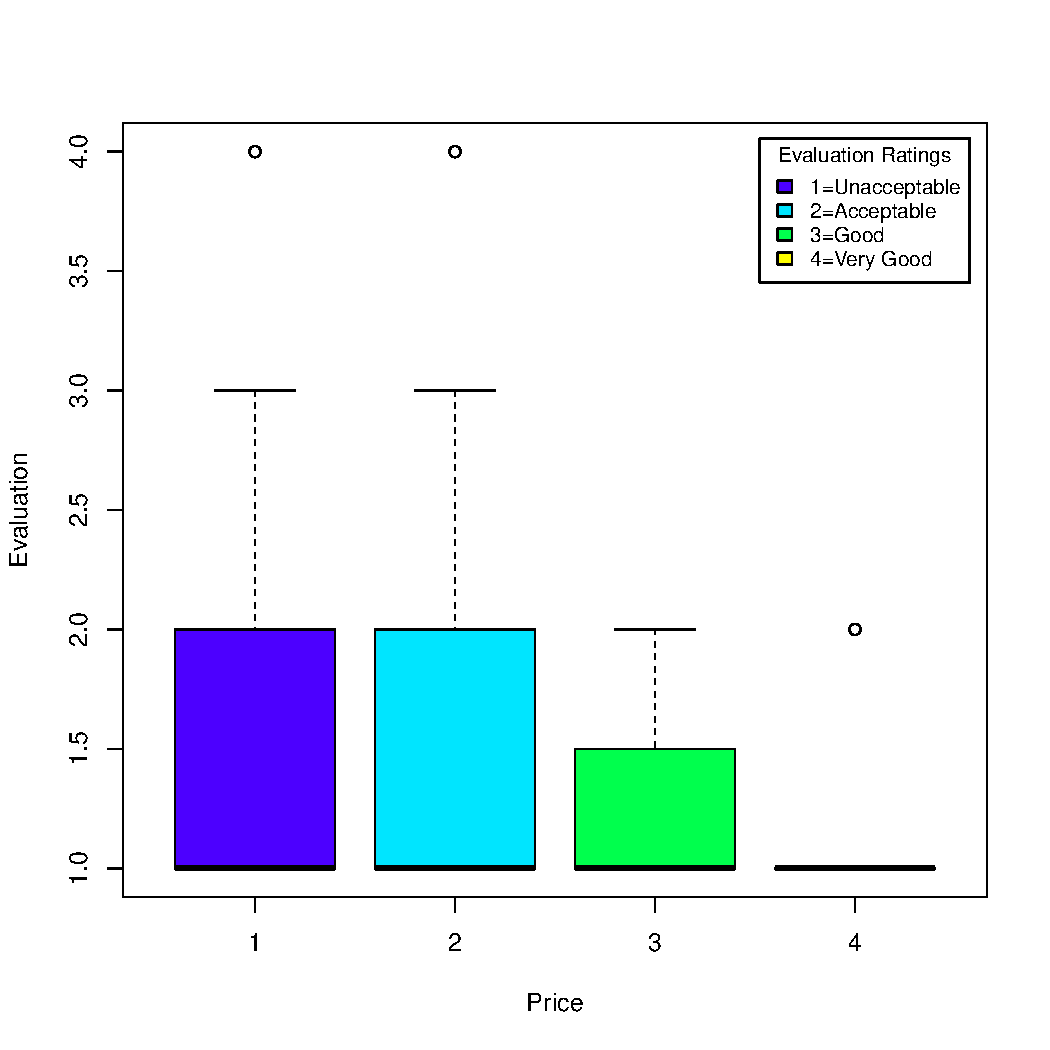
\includegraphics[width=\maxwidth]{figure/unnamed-chunk-7-1} 

\end{knitrout}
\emph{Price; 1 = Low 2 = Medium 3 = High 4 = Very High} 
\section{Modelling/ Classification}
The approach taken to modelling the data set was the random forest technique this approach was taken because it outputs a prediction matrix's of arbitrary size in this case there are 4 factors which are being predicted which result in a prediction matrix size 16.Random forest combines flexibility and power into a learning method as the entity uses only a small random percentage of the full dataset. Moreover, the technique used can handle extremely large datasets which might cause other models to fail.  Furthermore random forest is appropriate for missing data as well as categorical or continous details.
\subsubsection*{Dividing the dataset into training and testing subset}
The system sets the class label as a factor after being transformed to a Numeric Value
\begin{knitrout}
\definecolor{shadecolor}{rgb}{0.969, 0.969, 0.969}\color{fgcolor}\begin{kframe}
\begin{alltt}
\hlcom{#Setting the Label as a Factor avoid to regression to face matheatical errors }
\hlstd{nd}\hlopt{$}\hlstd{Evaluation} \hlkwb{<-} \hlkwd{as.factor}\hlstd{(nd}\hlopt{$}\hlstd{Evaluation)}
\end{alltt}
\end{kframe}
\end{knitrout}
The system begins with spliting the data into training and testing sets.
\begin{knitrout}
\definecolor{shadecolor}{rgb}{0.969, 0.969, 0.969}\color{fgcolor}\begin{kframe}
\begin{alltt}
\hlcom{#Importing the Correct Library}
\hlkwd{library}\hlstd{(caret)}
\end{alltt}


{\ttfamily\noindent\itshape\color{messagecolor}{\#\# Loading required package: lattice}}

{\ttfamily\noindent\itshape\color{messagecolor}{\#\# Loading required package: ggplot2}}\begin{alltt}
\hlcom{#splitting the data set in to 2 parts one for training and the other for testing}
\hlcom{#80 percent set is the traing}
\hlstd{inTrain} \hlkwb{<-} \hlkwd{createDataPartition}\hlstd{(}\hlkwc{y}\hlstd{=nd}\hlopt{$}\hlstd{Evaluation,}
                               \hlkwc{p}\hlstd{=}\hlnum{.8}\hlstd{,}\hlkwc{list}\hlstd{=}\hlnum{FALSE}\hlstd{)}
\hlcom{#defining the training set as the variable created above}
\hlstd{training} \hlkwb{<-} \hlstd{nd[inTrain,]}
\hlcom{#defining the testing data set from what is left over from the variable created above }
\hlstd{testing} \hlkwb{<-} \hlstd{nd [}\hlopt{-}\hlstd{inTrain,]}
\hlcom{#Performing a test to check the the total number of records both train/test are equal to the orgininal set}
\hlcom{#This should result in a display of true}
\hlkwd{nrow}\hlstd{(training)}\hlopt{+}\hlkwd{nrow}\hlstd{(testing)}\hlopt{==}\hlkwd{nrow}\hlstd{(nd)}
\end{alltt}
\begin{verbatim}
## [1] TRUE
\end{verbatim}
\end{kframe}
\end{knitrout}
The program creates a fit model on which the classification can begin
\begin{knitrout}
\definecolor{shadecolor}{rgb}{0.969, 0.969, 0.969}\color{fgcolor}\begin{kframe}
\begin{alltt}
\hlcom{#create the variable on which the evaluation is being predicted against all others }
\hlstd{fitModel} \hlkwb{<-} \hlkwd{train}\hlstd{(Evaluation} \hlopt{~} \hlstd{.,}\hlkwc{data}\hlstd{=training,}
                  \hlkwc{method}\hlstd{=}\hlstr{"rf"}\hlstd{,}\hlkwc{prox}\hlstd{=}\hlnum{TRUE}\hlstd{)}
\end{alltt}


{\ttfamily\noindent\itshape\color{messagecolor}{\#\# Loading required package: randomForest}}

{\ttfamily\noindent\itshape\color{messagecolor}{\#\# randomForest 4.6-12}}

{\ttfamily\noindent\itshape\color{messagecolor}{\#\# Type rfNews() to see new features/changes/bug fixes.}}

{\ttfamily\noindent\itshape\color{messagecolor}{\#\# \\\#\# Attaching package: 'randomForest'}}

{\ttfamily\noindent\itshape\color{messagecolor}{\#\# The following object is masked from 'package:ggplot2':\\\#\# \\\#\#\ \ \ \  margin}}\begin{alltt}
\hlcom{#Displaying the final model before the predictions}
\hlstd{fitModel}\hlopt{$}\hlstd{finalModel}
\end{alltt}
\begin{verbatim}
## 
## Call:
##  randomForest(x = x, y = y, mtry = param$mtry, proximity = TRUE) 
##                Type of random forest: classification
##                      Number of trees: 500
## No. of variables tried at each split: 6
## 
##         OOB estimate of  error rate: 1.52%
## Confusion matrix:
##     1   2  3  4 class.error
## 1 961   4  3  0 0.007231405
## 2   2 299  5  2 0.029220779
## 3   1   1 53  1 0.053571429
## 4   0   1  1 50 0.038461538
\end{verbatim}
\begin{alltt}
\hlstd{df_C} \hlkwb{<-} \hlkwd{classCenter}\hlstd{(training[,}\hlkwd{c}\hlstd{(}\hlnum{3}\hlstd{,}\hlnum{4}\hlstd{)],}
                    \hlstd{training}\hlopt{$}\hlstd{Evaluation,fitModel}\hlopt{$}\hlstd{finalModel}\hlopt{$}\hlstd{prox)}
\hlstd{df_C} \hlkwb{<-} \hlkwd{as.data.frame}\hlstd{(df_C)}
\hlstd{df_C}\hlopt{$}\hlstd{Evaluation} \hlkwb{<-} \hlkwd{rownames}\hlstd{(df_C)}
\end{alltt}
\end{kframe}
\end{knitrout}
Displaying the fitmodel
\begin{knitrout}
\definecolor{shadecolor}{rgb}{0.969, 0.969, 0.969}\color{fgcolor}\begin{kframe}
\begin{alltt}
\hlcom{#Getting the system to display the fit model}
\hlkwd{summary}\hlstd{(fitModel)}
\end{alltt}
\begin{verbatim}
##                 Length  Class      Mode     
## call                  5 -none-     call     
## type                  1 -none-     character
## predicted          1384 factor     numeric  
## err.rate           2500 -none-     numeric  
## confusion            20 -none-     numeric  
## votes              5536 matrix     numeric  
## oob.times          1384 -none-     numeric  
## classes               4 -none-     character
## importance            6 -none-     numeric  
## importanceSD          0 -none-     NULL     
## localImportance       0 -none-     NULL     
## proximity       1915456 -none-     numeric  
## ntree                 1 -none-     numeric  
## mtry                  1 -none-     numeric  
## forest               14 -none-     list     
## y                  1384 factor     numeric  
## test                  0 -none-     NULL     
## inbag                 0 -none-     NULL     
## xNames                6 -none-     character
## problemType           1 -none-     character
## tuneValue             1 data.frame list     
## obsLevels             4 -none-     character
## param                 1 -none-     list
\end{verbatim}
\end{kframe}
\end{knitrout}
Building the prediction model
\begin{knitrout}
\definecolor{shadecolor}{rgb}{0.969, 0.969, 0.969}\color{fgcolor}\begin{kframe}
\begin{alltt}
\hlcom{#Test the model for this run}
\hlstd{pred} \hlkwb{<-} \hlkwd{predict}\hlstd{(fitModel, testing)}
\hlstd{testing}\hlopt{$}\hlstd{correctPred} \hlkwb{<-} \hlstd{pred}\hlopt{==}\hlstd{testing}\hlopt{$}\hlstd{Evaluation}
\end{alltt}
\end{kframe}
\end{knitrout}
Retriving the Result
\begin{knitrout}
\definecolor{shadecolor}{rgb}{0.969, 0.969, 0.969}\color{fgcolor}\begin{kframe}
\begin{alltt}
\hlcom{#Assigning and displaying the results}
\hlstd{results} \hlkwb{<-} \hlkwd{table}\hlstd{(pred,testing}\hlopt{$}\hlstd{Evaluation)}
\hlstd{results}
\end{alltt}
\begin{verbatim}
##     
## pred   1   2   3   4
##    1 237   2   0   0
##    2   4  73   0   1
##    3   0   1  13   0
##    4   0   0   0  12
\end{verbatim}
\end{kframe}
\end{knitrout}
Testing the values to see what the Accuracy is
\begin{knitrout}
\definecolor{shadecolor}{rgb}{0.969, 0.969, 0.969}\color{fgcolor}\begin{kframe}
\begin{alltt}
\hlcom{#Assinging the accuracy and displaying it}
\hlstd{accuracy} \hlkwb{<-} \hlkwd{sum}\hlstd{(}\hlkwd{diag}\hlstd{(results))} \hlopt{/} \hlkwd{sum}\hlstd{(results)} \hlopt{*} \hlnum{100}
\hlstd{accuracy}
\end{alltt}
\begin{verbatim}
## [1] 97.66764
\end{verbatim}
\end{kframe}
\end{knitrout}

\section{Improving Performance}









































%Include the bar chart photos please
%ask Eyad about the scatter plot of inthe second attempt.


%ask if line 203 is correct

%improvment bit 
%Random forest contains several parameters that can be tuned to improve the performance. However, here we will only try to vary the number of trees and see if this makes any difference in the classification accuracy:Fit model, vary number of trees, and visualise results: Check out LAB 4

\end{document}
